\documentclass[a4paper,11pt]{book}

/maxwit/document/texbuild/style.tex

\title{g-bios Users' Manual}
\author{MaxWit~魔鬼训练营}

%\renewcommand{\baselinestretch}{1.3}
\linespread{1.3}

\begin{document}
\maketitle

\frontmatter
\tableofcontents

\mainmatter
\chapter{Getting Started with g-bios}

\section{Introduction to MaxWit g-bios}
%\section{g-bios: An Open Source Bootloader Project}
~MaxWit~开放实验室(~MaxWit Open Lab~)是由多家公司资助成立的,致力于研发开源项目和探讨软件开发技术的公益性组织。2008年1月正式成立于上海浦东张江高科,目前开放实验室成员主要来源于~Google~、~Intel、~ ~TI~、~AMD~、华为、~Cisco~、飞利浦等公司资深研发人员以及清华、浙大、上交大、中科院等科研院校的师生。

~MaxWit~ ~g-bios~(以下简称~g-bios~)是由~MaxWit~开放实验室和开源社区共同研发的一个~Bootloader~,或者说是一个嵌入式系统的~BIOS,~相当于PC机的~BIOS~+~Bootloader~。~g-bios~不但借鉴了几乎所有主流~BSP/BIOS/Bootloader~的优点,而且加入不少独创的特性,包括(但不局限于):
%\begin{enumerate}[1)]\setlength{\itemsep}{-\itemsep}
\begin{enumerate}\setlength{\itemsep}{-\itemsep}
\item 自动检测有待烧录的~image~文件类型,并智能自动烧录。
\item 支持多种文件系统,包括~YAFFS2、JFFS2、CRAMFS、UBI、NFS~等。
\item 支持两种用户界面:~GUI~(类似传统~PC BIOS~)和命令行模式(面向嵌入式系统)。
\item 命令行自动补全(~Tab~)键及历史记录(上、下键)支持。
\item ~Flash(MTD)~分区支持,帮助~Linux、Android~内核识别分区。
\item 自动设置~Linux~内核启动参数(~Linux kernel command line~),极大地降低了参数设置的复杂度并减少了启动出错的概率。当然,同时也支持手动设置,以满足特殊要求。
\item 常用命令具有记忆功能。如~boot~命令,它能记住用户输入的参数,以后只需简单输入~boot~即可。
\item 引入全新的架构及~NB~(~Never~ ~Burn~ ~Down~,烧不死)技术。核心设计思想是:把~g-bios~分为上半部分和下半部分,上半部分以最小的代码量完成~CPU~和~Memory~的初始化,并实现引导下半部分的功能;下半部分为~g-bios~主体。上半部分设计简单,调试周期短,完成后就固化在特定的引导区中不再更改;开发人员可在没有仿真器的情况下大胆开发下半部分代码(即~g-bios~主体),事实上,只需一根串口数据线应能轻松完成整个~g-bios~的开发。启动代码的地址无关性带来的麻烦?没有了!因为~bug~或不小心改错了代码,甚至是数据线连接问题而导致启动黑屏?也不可能出现了!在调试完成并正试发布的产品时,若有必要,也可将上下两部分可合成一个整体——只需一个命令重新编译即可。
\item 优秀的子系统设计,包括:中断、网络、~Flash、USB~子系统,等等。
\item 集成类似~PC~机版本的~Video BIOS~。
%\item 支持基于龙芯的~PC~机及嵌入式系统。
\item 完美支持~Google Android~操作系统,简化~Android~的系统移植过程。
\item 支持图形化配置,不但让新手很容易上手,而且使~g-bios~的移植和开发过程变得更简单。
\end{enumerate}
更多详情,请登录项目主页~http://maxwit.googlecode.com~或~ChinaUnix~论坛(~http://linux.chinaunix.net/bbs~)上的~g-bios~版块。

\section{Getting the Source Code}
请确认~git~(一个版本管理软件)已经安装,然后执行如下命令:
\begin{lstlisting}[language=bash,numbers=none]
$cd
$git clone git://github.com/maxwit/g-bios.git
\end{lstlisting}
此时会在当前目录(方便描述起见,假定为~HOME~目录)下将会创建一个名为 ``~g-bios~''的目录,该目录中为~g-bios~源码。
%\section{如何参与~g-bios~开发}
%~g-bios~开源社区采用~maillist~和~bbs~相结合的方式,任何人都可以通过这两种方式把自己的代码递交给~g-bios~项目维护者。若对文档有任何疑问或改进也可联系我们。
%  \begin{table}[htbp]
%  \centering
%  \setlength{\parindent}{0pt}
%  \begin{tabular}{|c|c|}
%  \hline
%  ~g-bios~论坛 &\small ~http://linux.chinaunix.net/bbs/forum-70-1.htm~ \\
%  \hline
%  ~g-bios~邮件列表 &\small ~maxwit@googlegroups.com~ \\
%  \hline
%  ~g-bios~项目维护者 &\small~Conke Hu~ $<$~conke.hu@gmail.com~$>$ \\
%					 &\small~Tiger Yu~ $<$~tigerflying.yu@gmail.com~$>$ \\
%					 &\small~Fleya Hou~ $<$~fleya.hou@gmail.com~$>$ \\
%  \hline
%  文档编辑 &\small  \\
%  \hline
% \end{tabular}
% \end{table}

\section{g-bios Architecture}

\section{Source Directory Tree}
\begin{lstlisting}[language=bash, numbers=none]
$ ls ~/g-bios/
bh  build  doc  include  Makefile  th
\end{lstlisting}

\begin{equation*}
\text{g-bios}
\left\{
	\begin{aligned}
	&\text{th: stage 1~代码} \\
	&\text{bh: stage 2~代码,即~g-bios~上半部分启动代码} \\
	&\text{Makefile:} 整个~g-bios~项目的顶层~Makefile~ \\
	&\text{include:头文件(stdio.h, string.h, g-bios.h等)} \\
	&\text{doc:使用开发手册} \\
	&\text{build:与编译相关文件夹(配置文件,编译规则)} \\
	\end{aligned}
\right.
\end{equation*}


~bh~目录:
\begin{lstlisting}[language=bash, numbers=none]
$ ls ~/g-bios/bh
app  arm  base  driver  filesys  lib  Makefile  mm
\end{lstlisting}

\begin{equation*}
\text{bh: stage 2}
\left\{
	\begin{aligned}
	&\text{app:g-bios~应用程序、命令所在目录(ping, ls, reboot~等)} \\
	&\text{arm:arm~体系结构相关代码} \\
	&\text{base:g-bios~下半部分公共文件夹(main, shell, sysconfig~等)} \\
	&\text{driver: 驱动程序源码,通用~driver~} \\
	&\text{filesys:文件系统相关源码} \\
	&\text{lib:库文件(stdlib, string, net等)} \\
	&\text{mm:内存管理文件夹(内存分配函数代码等)}
	\end{aligned}
\right.
\end{equation*}

~app~目录

\begin{lstlisting}[language=bash, numbers=none]
$ ls ~/g-bios/app
boot  flash  led  Makefile  memory  misc  net  serial  shell  sysconf
\end{lstlisting}
将不同功能的~application~分成类,置于不同的文件夹下。每个文件下都有一个~Makefile~文件。从文件夹的命名就可知道其文件夹下有哪些文件。~app~文件下的每个~.c~文件都对应~g-bios~中的某个命令,文件名就是~g-bios shell~中的命令名。
\begin{equation*}
\text{bh/app}
\left\{
	\begin{aligned}
	&\text{boot:引导程序(boot kernel or reboot, etc)} \\
	&\text{flash:~flash~操作相关~app~} \\
	&\text{led:控制~led~灯程序} \\
	&\text{Makefile} \\
	&\text{memory:memory~操作函数} \\
	&\text{misc:杂项程序} \\
	&\text{net:网络程序} \\
	&\text{serial:串口程序} \\
	&\text{shell: clear, ls, etc} \\
	&\text{sysconf: configure~程序}
	\end{aligned}
\right.
\end{equation*}

目前~g-bios~仅支持~arm~体系结构的处理器,因此仅有~arm~目录。
\begin{lstlisting}[language={SH},numbers=none]
$ ls ~/g-bios/bh/arm/
arm_heap.c  at91sam926x  exception.c  g-bios-bh.lds  head.S  lib  Makefile  omap3530  s3c24x0  s3c6410  udelay.S
\end{lstlisting}

\begin{equation*}
\text{bh/arm}
\left\{
	\begin{aligned}
	&\text{arm\_heap.c:heap init} \\
	&\text{at91sam926x} \\
	&\text{exception.c:exception handle} \\
	&\text{g-bios-bh.lds:编译~bh~所需的链接脚本。} \\
	&\text{head.S:stage 2~入口} \\
	&\text{lib:arm~体系结构相关库文件} \\
	&\text{Makefile}\\
	&\text{omap3530}\\
	&\text{s3c24x0}\\
	&\text{s3c6410}\\
	&\text{udelay.S:udelay}
	\end{aligned}
\right.
\end{equation*}
其中~at91sam926x~、~s3c24x0~、~s3c6410~为平台相关代码:包括~soc~相有关的driver~,~board~级初始化代码。

嵌入式开发要了解的几个概念:板级,~SOC~级,~CPU~级,~CPU core~级。板级:与硬件开发板的布线有关。现在嵌入式处理器,通常将~SOC~级,~CPU~级,~CPU core~级做成一颗芯片。也就是所说的~SOC~,例如~s3c6410~,~s3c2440~,~at91sam9261~等这就是一个~SOC~。每个芯片公司将一个常用的外设芯片集成在一个~cpu~芯片里,就生产出了自己的~SOC~处理器芯片。这也就是说不同的~SOC~,他们所集成的外设可能会不一样。因此对于不同的~SOC~,他们的相对的处理代码也就可能不一样了。~SOC~里集成了外设,所以也可将~SOC~叫做~platform~或``板子''。~cpu core~也就是所说的体系结构例如:~arm v5~,~arm v6~,~arm v7~,~core 2~等。~cpu~就将~cpu core~,~MMU~,~cache~等等集成在一起的芯片,不同的~CPU~,它们的~cache~个数、大小可能不同,因此处理~cpu~级的程序代码也可能不同。(例如:~arm 9~,~arm 11~,~cotex-a8~等)。其它厂商可以在此基础上加入一此外设从而制造处一个~SOC~。因此,对于不同的~SOC~,他们的~cpu~和~cpu core~可能相同(~s3c2410~,~s3c2440~他们的都是~arm 9~系列~cpu~,因此他们的~cpu~和~cpu-core~就是一样)。

有了以上基础后再来看~ARCH~相关的目录结构就十分简单了。~s3c6410~,~at91sam926x~,~s3c24x0~为不同~cpu~的处理程序,里含各个~SOC~处理的相关的代码。~*.c~,~*.s~体系结构公共相关的代码。~lib~体系结构相关库文件。

~th~目录:
\begin{lstlisting}[language={SH}]
$ ls ~/g-bios/th/
arm  base Makefile
\end{lstlisting}
~g-bios~上半部分启动程序,~arm~目录与上面所讲的~arm~目录类似, 里不再重述。
~base~目录上半部分与体系结构无关代码(~main, ymodem, kermit~等)。

driver~目录:
\begin{lstlisting}[language=bash, numbers=none]
$ ls ~/g-bios/driver
flash  gpu  Makefile  mmc  net  uart
\end{lstlisting}
不同外设的驱动程序源码。

\begin{equation*}
\text{driver}
\left\{
	\begin{aligned}
	&\text{flash:flash驱动程序(nand flash, nor flash, dataflash等)}\\
	&\text{gpu:显卡驱动程序(lcd等)}\\
	&\text{mmc:mmc相关驱动(sd卡等)}\\
	&\text{net:net相关驱动(dm9000网卡驱动,cs8900驱动,协议栈等)}\\
	&\text{uart:串口相关驱动。}
	\end{aligned}
\right.
\end{equation*}

\chapter{Building g-bios}
\section{g-bios Configuration}
在~g-bios~源码目录下有~Makefile~文件,和内核一样,进入目录后,先执行~make xxxx\_defconfig~(~xxxx~指的是~SOC~的名称,例如~S3C6410\_defconfig~或者~at91sam9261\_defconfig, g-bios~所支持的~SOC~的默认配置文件位于~g-bios~源码~build/configs/arm~目录下),用默认的选项编译~g-bios~,然后执行~make~进行编译,如需要将编译产生的~image~文件拷贝到~tftpboot~目录下,还需要执行~make install~命令。如果需要修改默认的编译选项,可以直接执行~make menuconfig~,在随后出现的~GUI~中进行配置。
\begin{lstlisting}[language=bash, numbers=none]
$ cd g-bios
$ make s3c6410_defconfig
$ make
$ make install
\end{lstlisting}
或者
\begin{lstlisting}[language=bash, numbers=none]
$ cd g-bios
$ make menuconfig
$ make
$ make install
\end{lstlisting}


~g-bios~的~configure~程序支持图形界面的配置,使用者可在图形界面的配界相应功能。接下来分析一个各个配置选项的功能作用。

~Platform~:	~g-bios~运行的~platform~,可以是~at91sam9263~、~at91sam9261~、~s3c2410~、~s3c2440~或~s3c6410~等,这是目前~g-bios~支持的几个~Platform~。~Toolchain~:编译~g-bios~源码所选用的编译工具,默认使用的是~lablin~源码包编译生成的~toolchain~,也可以手工修改为系统上已有的~toolchain~(注:~Toolchain~要支持~EABI~)。~Image Patch~编译~g-bios~后生成的image路径,默认为/var/lib/tftpboot目录。Server IP服务器IP,local IP开发板IP,将二者设为同一网段。此二项,也可不配。~MAC Addr~此项不用理会,~Nfs Path~:~g-bios~引导内核时,如用~nfs~加载~rootfs~时,指定~rootfs~路径,默认路径~$\sim$/maxwit/rootfs~。~Flash ECC mode~选择~ECC~校验模式(硬件ECC,软件ECC,也可不使用ECC)。~IRQ/Polling Mode~ g-bios使用中断模式还是非中断模式(Polling)。

g-bios~配置程序所完成的功能:
\begin{table}[htbp]
\centering
\setlength{\parindent}{0pt}
\begin{tabular}{|c|l|l|}
\hline
类别 & \multicolumn{1}{|c|}{选项} & \multicolumn{1}{|c|}{功能说明} \\ \hline
\multirow{3}{*}{general} & Platform & g-bios运行的目标Platform \\ \cline{2-3}
		& TooLchain & 编译~g-bios~的编译工具 \\ \cline{2-3}
		& Image Path & 编译生成image的目录 \\ \hline
\multirow{4}{*}{Network} & Server IP & 服务器IP \\ \cline{2-3}
		& Local IP & 目标机IP \\ \cline{2-3}
		& MAC addr & MAC地址\\ \cline{2-3}
		& NFS root path &  lablin的rootfs路径\\ \hline
\multirow{3}{*}{~Flash ECC Mode~}   & Hardward & 支持硬件ECC\\ \cline{2-3}
		& Software & 软件ECC\\ \cline{2-3}
		& None & 无ECC较验\\ \cline{2-3}
\multirow{2}{*}{~IRQ/Polling Mode~} & IRQ Enabled & 支持中断 \\ \cline{2-3}
		& Polling Mode & 查询模式(非中断)\\ \hline
\end{tabular}
\end{table}

\subsection{Configuration Options}
\begin{itemize}
\item Gerneral
\item Tophalf
\item Uart
\item Memory
\item Flash
\item NetWork
\item Interrupt
\item Logo
\item Boot
\end{itemize}

\section{``make'' and ``install''}
上面通过~configure~配置的~g-bios~编译特性,生成了~Makefile~。本节将编译~g-bios~。
\begin{lstlisting}[language=bash,numbers=none]
$ make
$ make install
\end{lstlisting}
编译后会在/var/lib/tftpboot(~configure~中配置的~Image Path~)目录下生成~g-bios-th.bin~和~g-bios-bh.bin~二个文件。

\chapter{Burning g-bios}

\section{Overview}
\subsection{Burning Top-Half}
g-bios~上半部分的烧录方法与其他的~bootloader~一样,都依赖于具体的板子,请大家参考板子的手册烧录~TH。
g-bios~上半部主要是~Load~下半部,为下半部服务。Load BH~的方式有如下几种:
\begin{enumerate} \setlength{\itemsep}{-\itemsep}
\item 从串口下载下半部并运行
\item 从~Flash~上~Load~下半部并运行
\item 自动检测~Flash~上的下半部是否存在,若存在则默认从~Flash~上~Load~下半部并运行,否则等待从串口~Load~。
\end{enumerate}

\subsection{Burning Bottom-Half}
上电或重起后,连接任意键可即可进入~g-bios TH~的引导菜单。若不按键刚~TH~默认从~Nand Flash~中~Load BH~并执行将执制权交给~BH~。通过~TH Load BH~的菜单如下所示:
\begin{figure}[H]
\centering
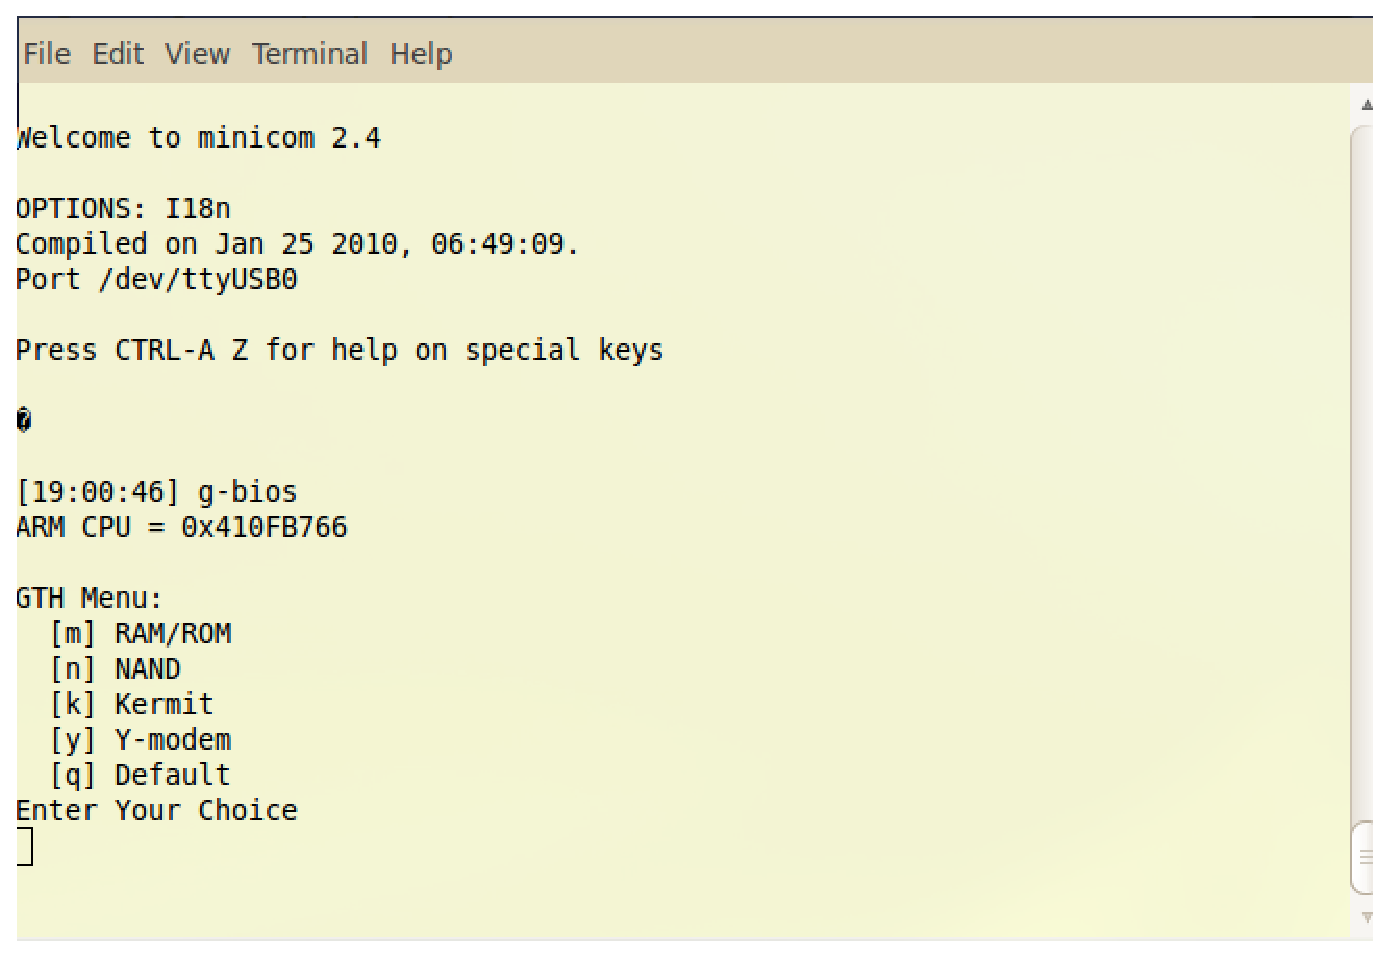
\includegraphics[width=0.8\textwidth]{image/min_01.eps}
\end{figure}
选择不同的选择即可以不同的方式~Load BH~。以~Kermit~和~Minicom~为例从串口引导~g-bios bh~。
\begin{enumerate} \setlength{\itemsep}{-\itemsep}
\item Ymode:(注意:~minicom~在以下过程中要求使用速度很快。)
	\begin{enumerate} \setlength{\itemsep}{-\itemsep}
	\item 连接电源,串口线(开发板上的~COM1~),网线。
	\item 打开~minicom~软件。
	\begin{lstlisting}[language=c,numbers=none]
	$ minicom
	\end{lstlisting}
	\item 按下空格键(一直接)。打开电源开关。
	\begin{figure}[H]
	\centering
	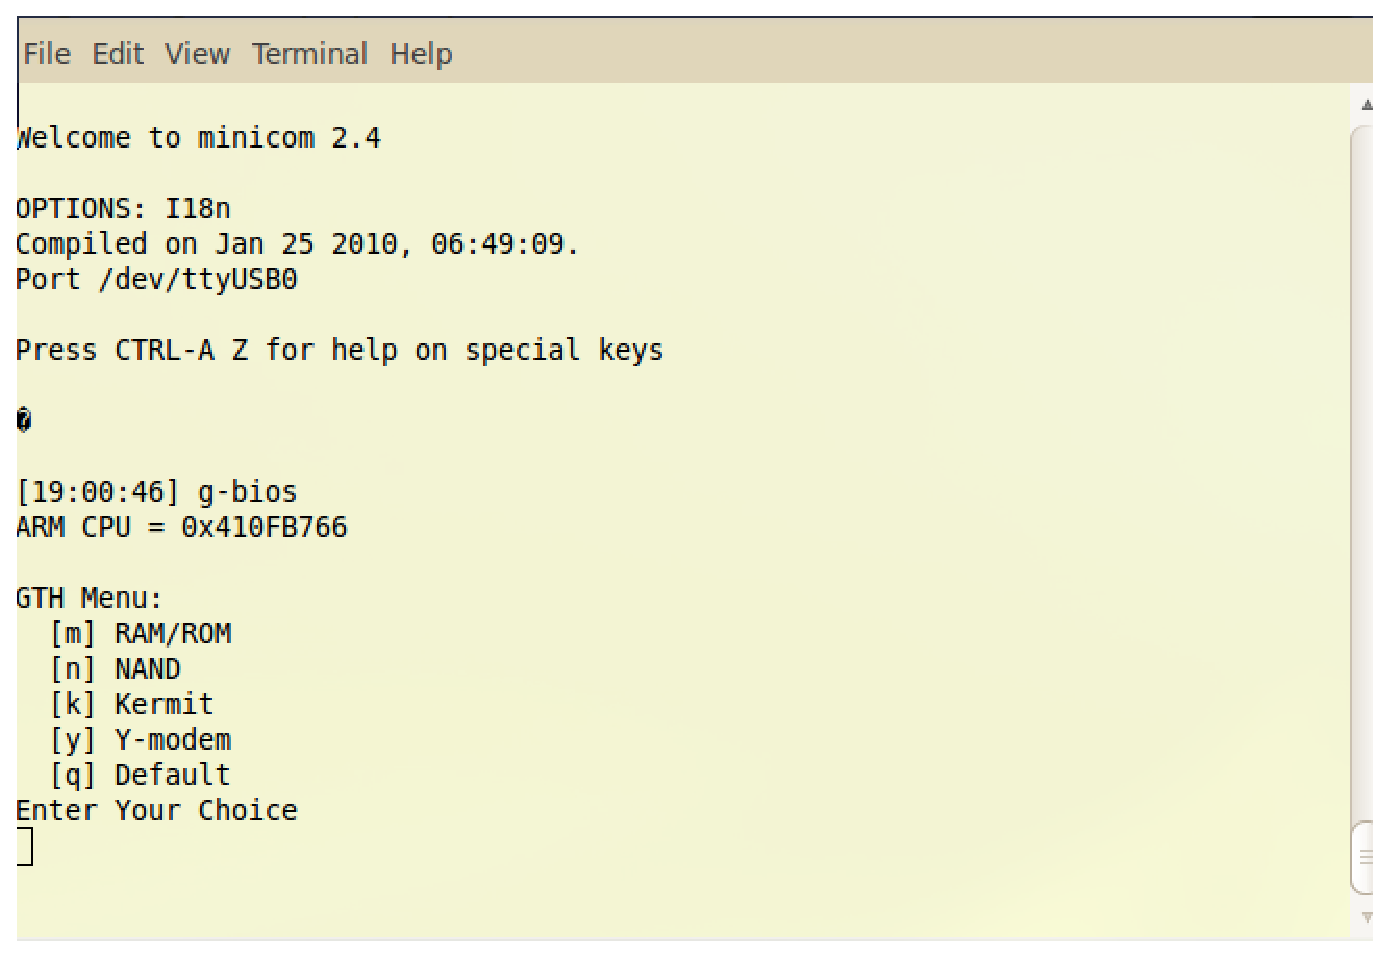
\includegraphics[width=0.8\textwidth]{image/min_01.eps}
	\end{figure}
	\item 按下'Y'键
		\begin{figure}[H]
		\centering
		\includegraphics[width=0.8\textwidth]{image/min_02.eps}
		\end{figure}
	\item 同时按下``Ctrl'' + 'a', 再按's'.
		\begin{figure}[H]
		\centering
		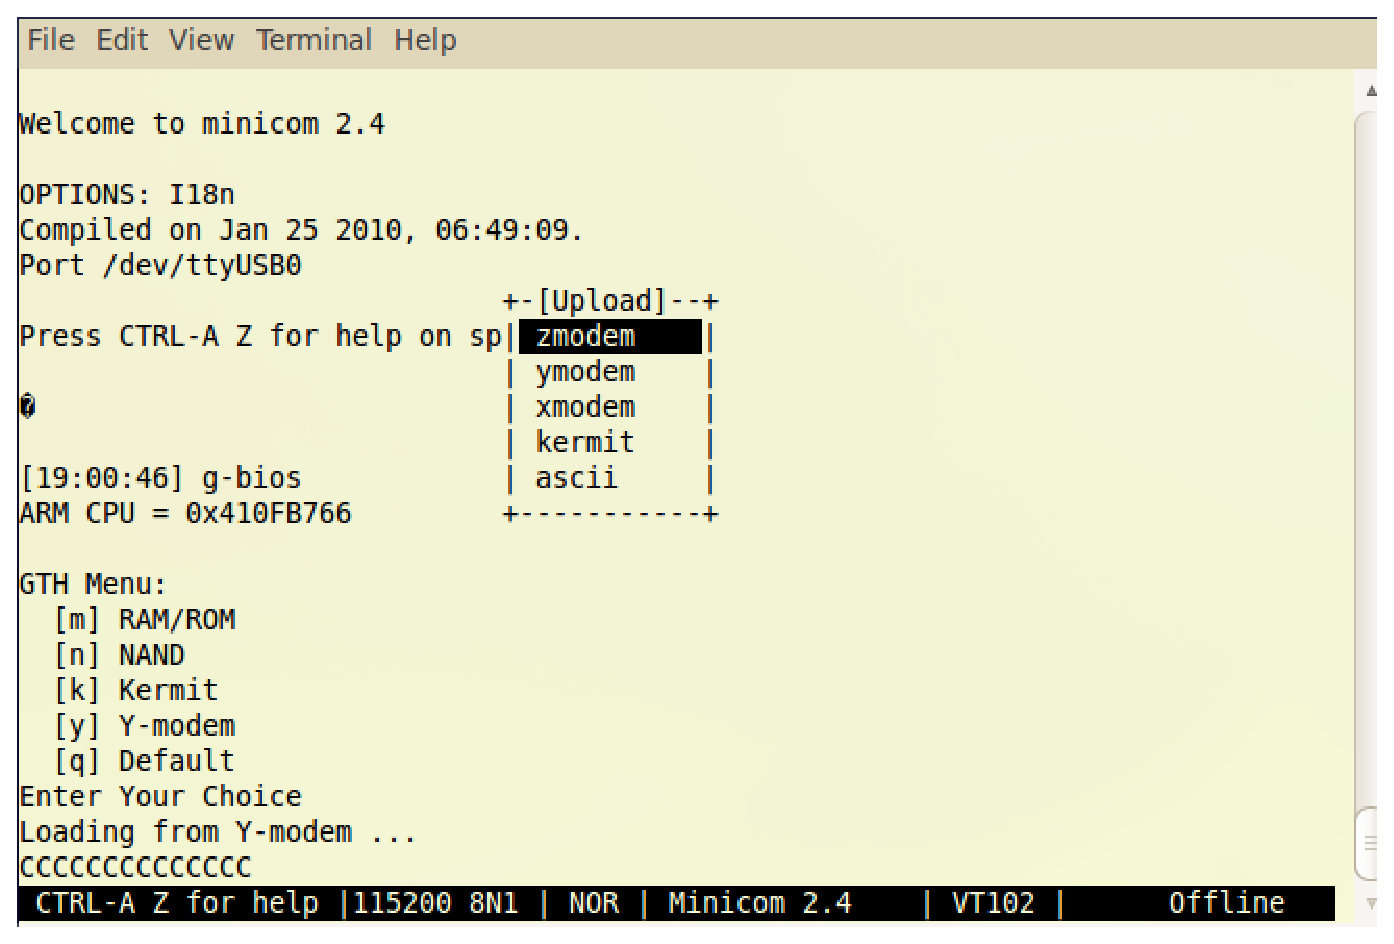
\includegraphics[width=0.8\textwidth]{image/min_03.eps}
		\end{figure}
	\item 用方向键选择~``ymode''~,回车。
		\begin{figure}[H]
		\centering
		\includegraphics[width=0.8\textwidth]{image/min_04.eps}
		\end{figure}
	\item 选择~``Okay''~,回车。
		\begin{figure}[H]
		\centering
		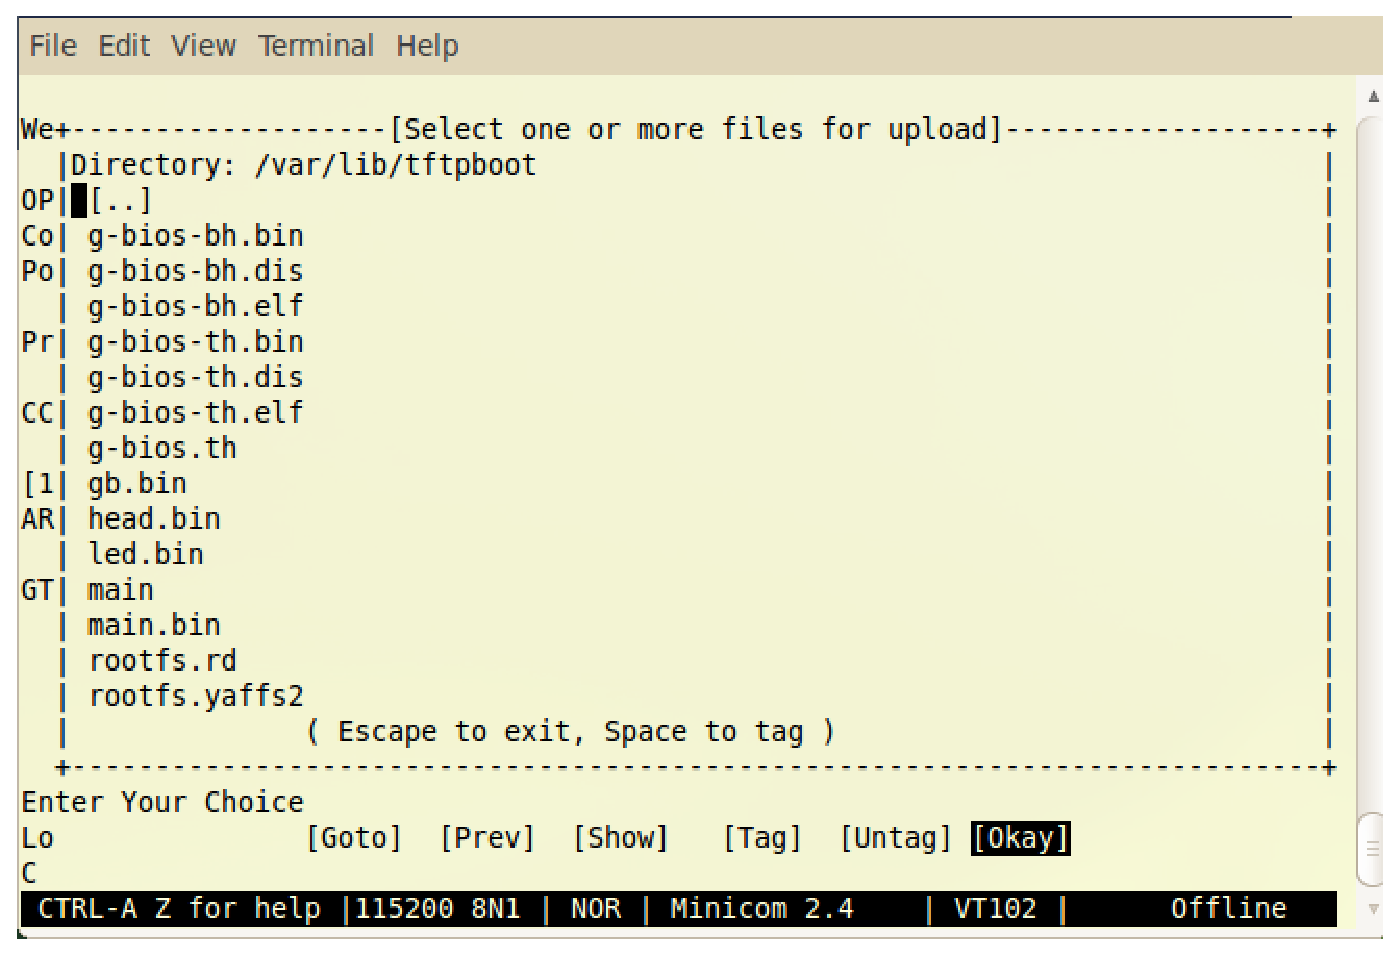
\includegraphics[width=0.8\textwidth]{image/min_05.eps}
		\end{figure}
	\item 输入~/var/lib/tftpboot/g-bios-bh.bin~。回车。此处输入的为~g-bios-bh.bin~文件的路径,可视具体情况更改。
		\begin{figure}[H]
		\centering
		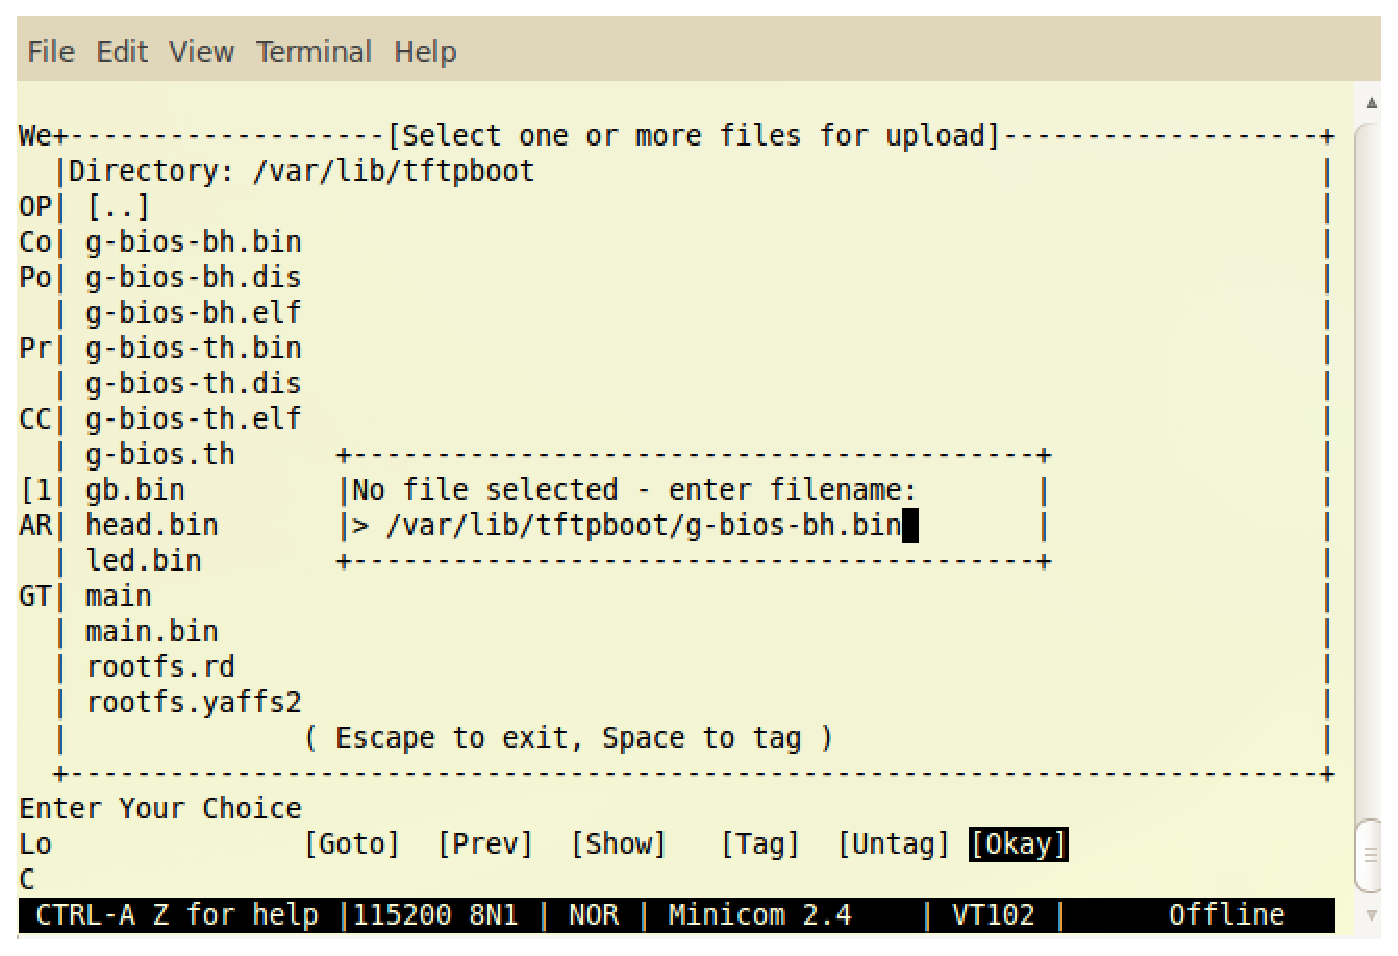
\includegraphics[width=0.8\textwidth]{image/min_06.eps}
		\end{figure}
	\item 开发传输文件,传送完成后如下图所示。再次回车。即可进入~g-bios Shell~。
		\begin{figure}[H]
		\centering
		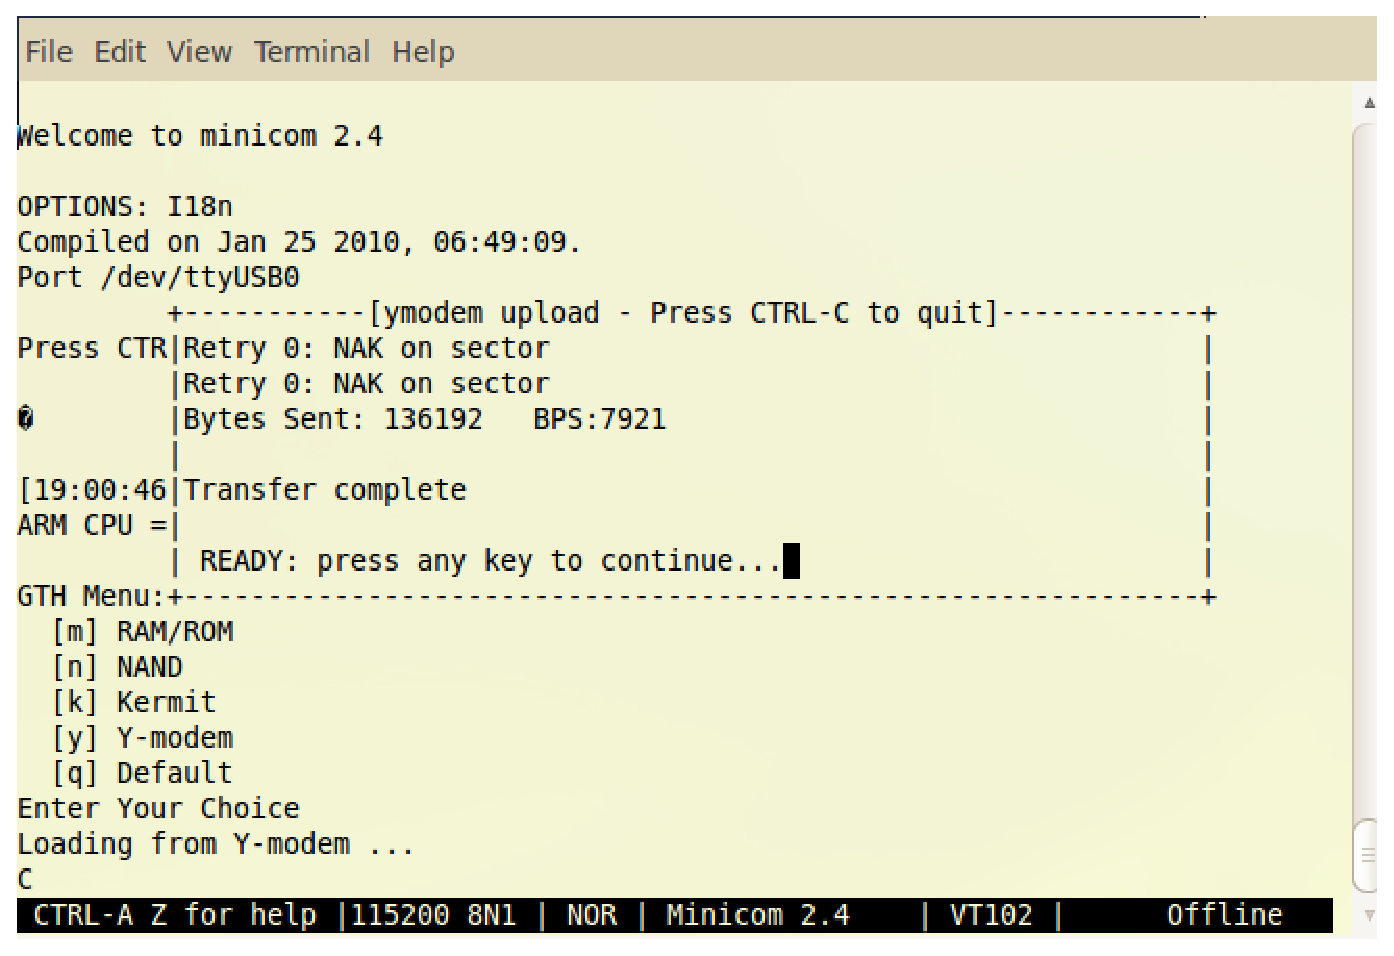
\includegraphics[width=0.8\textwidth]{image/min_07.eps}
		\end{figure}
	\item 进入~g-bios Shell~。如图所示。
		\begin{figure}[H]
		\centering
		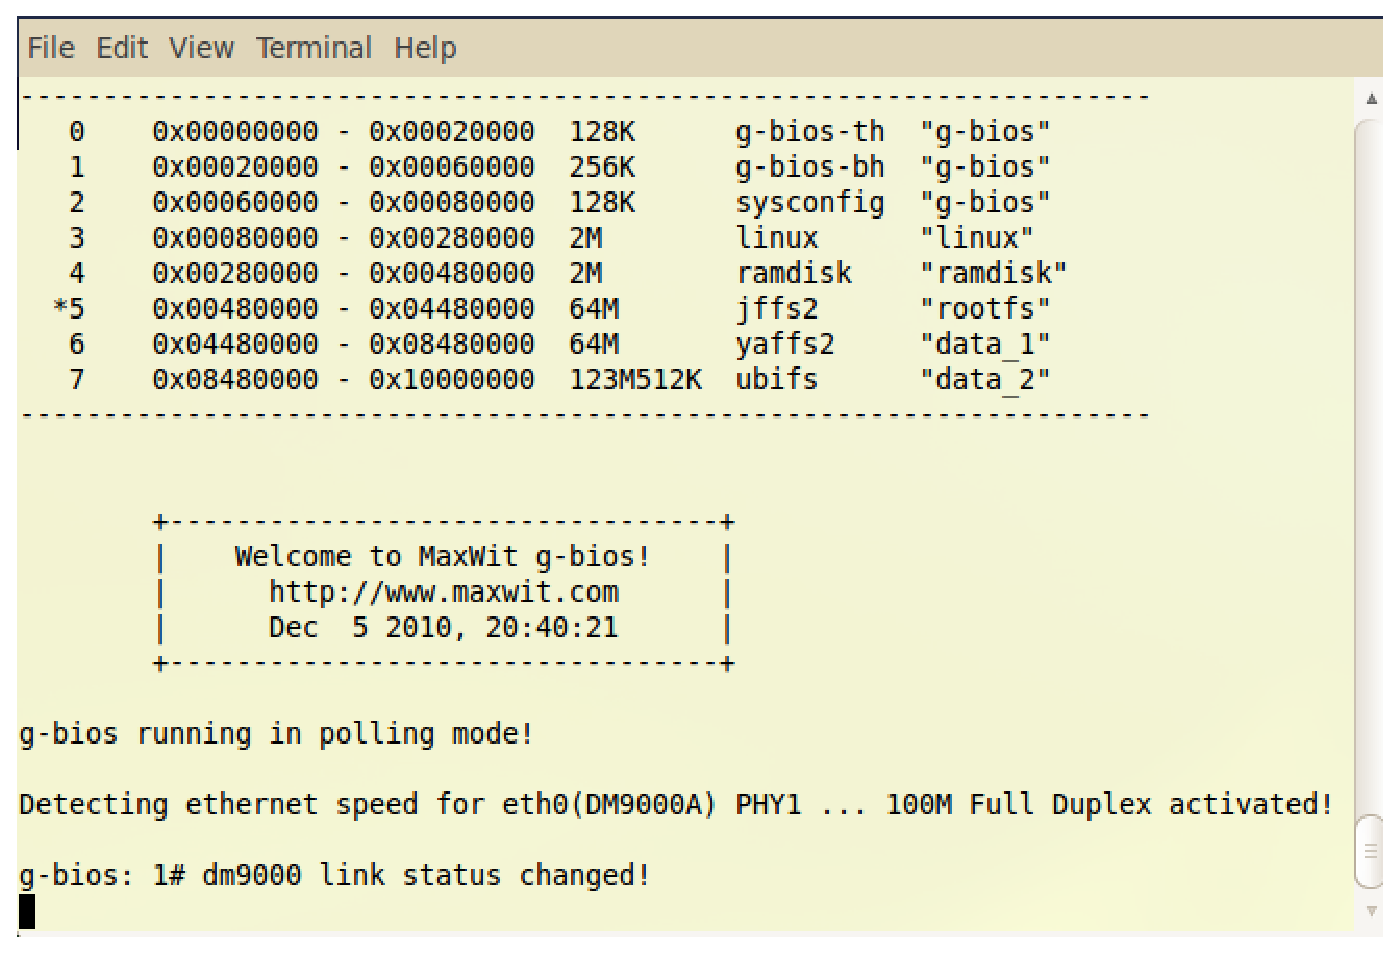
\includegraphics[width=0.8\textwidth]{image/min_08.eps}
		\end{figure}

	如果上述操作失败,以返回第三步(c步)重复操作,在第'f'步,不再重新输入,而是直接回车。
	\end{enumerate}
\item Kermit
\end{enumerate}
\noindent 第一步,先启动上半部,使用串口线将开发板上的~COM1~口和~PC~机的~COM~口连接、并用网线连接开发板和~PC~机,在~Host~端打开~kermit~\\
\begin{lstlisting}[language=bash,escapeinside=``]
$cd /var/lib/tftpboot
$kermit
C-kermit>c (`回车`)
\end{lstlisting}
\noindent 第二步,再按下开发板~Reset~键,将会进入~g-bios~上半部的启动界面(如图)\\

\begin{figure}[t]
\centering
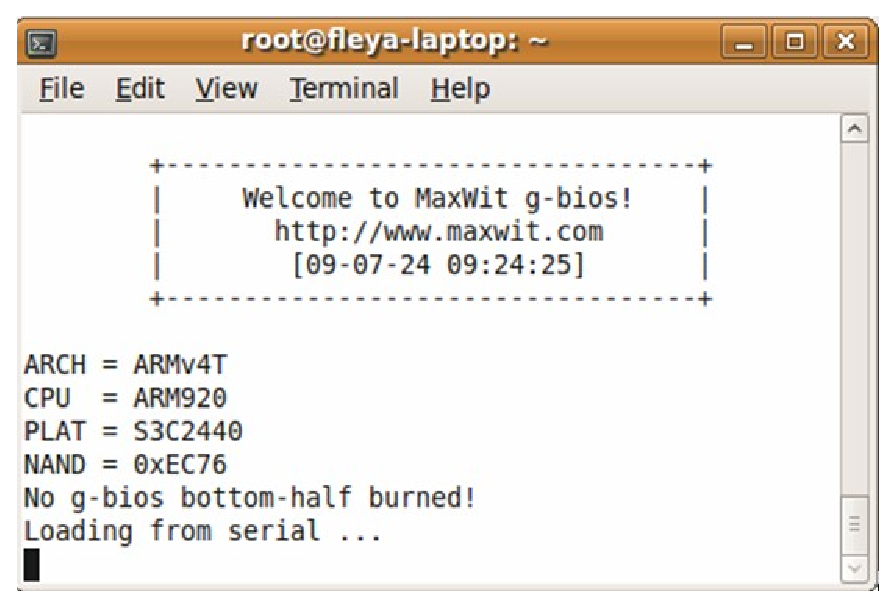
\includegraphics[width=5in]{image/step2.eps}
\end{figure}

\noindent 注:~g-bios~的上半部会自动检测~Flash~上是否已烧录下半部~g-bios-bh.bin~,若下半部已烧录则直接从~Flash~上将下半部~Load~到~Sdram~并运行,若未烧录则如上图所示,提示下半部未烧录,并需要通过从串口~Load~下半部并启动。下半部支持通过网络和串口两种方式烧录指定文件到~Flash~中。也在上半部启动过程中按任意键启动串口~Load~的功能.

\noindent 第三步,选择``k''回车, 然后同时按下``CTRL''和``\textbackslash''键, 再按下``c''\\

\begin{figure}[H]
\centering
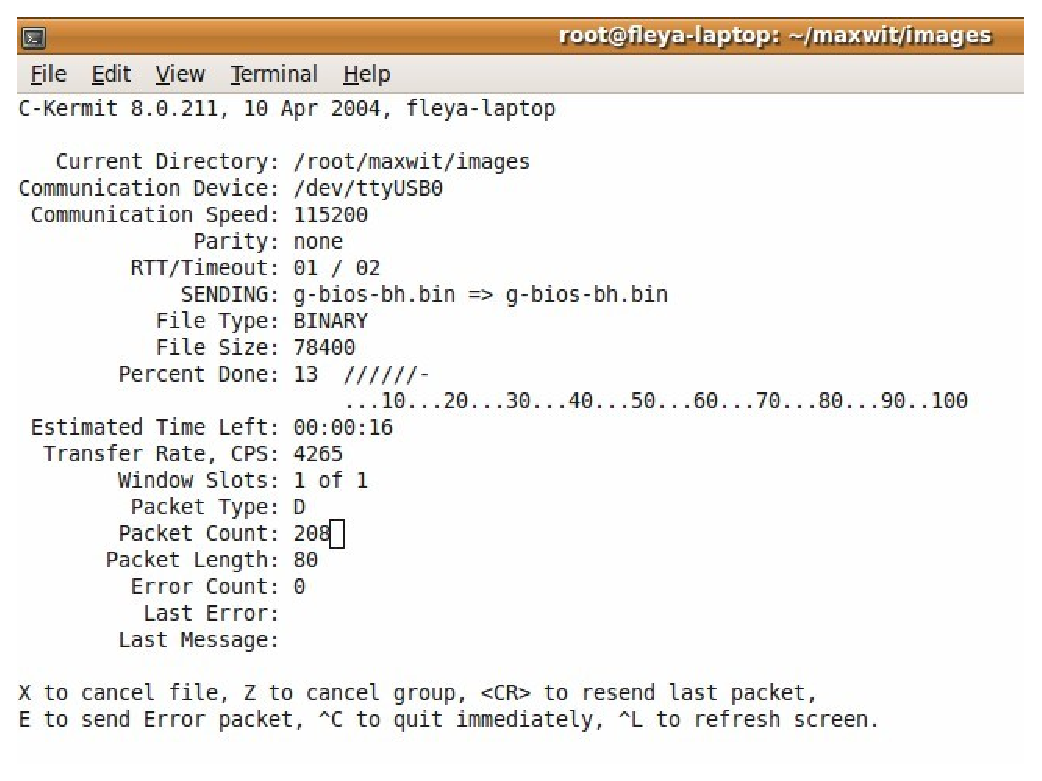
\includegraphics[width=5in]{image/step3.eps}
\end{figure}

\begin{lstlisting}[language=bash,numbers=none]
C-Kermit> send g-bios-bh.bin
\end{lstlisting}
进入~g-bios~下半部的启动界面,按任意键进入~g-bios~的命令行,否则~g-bios~将会自动~load kernel~并启动(如图)

\begin{figure}[H]
\centering
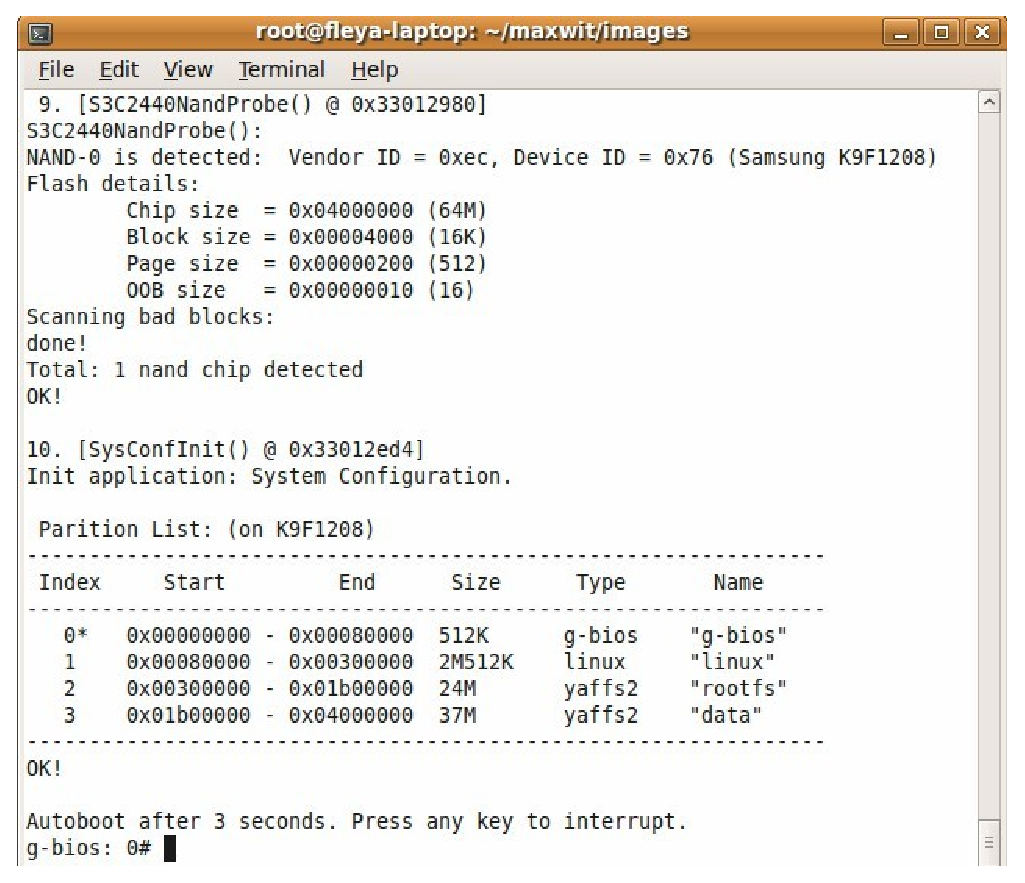
\includegraphics[width=5in]{image/step4.eps}
\end{figure}

\section{Burning g-bios with SD Card}
S3C64XX and S5P as cases

\begin{enumerate}
\item Write TH Image to SD Card
\item Booting g-bios TH from SD
\item Load BH to RAM
\item Burning TH and BH
\end{enumerate}

\chapter{g-bios Commands Reference}

%\section{Add New Commands}
%g-bios添加命令规范。
%\begin{lstlisting}
%static char app_option[][CMD_OPTION_LEN] = {};
%
%#include <getopt.h>
%
%int getopt(int argc, char *argv[], const char *optstring, char **arg);
%\end{lstlisting}

boot command design ..

\section{OS引导}
见第五章?
\begin{table}[H]
\setlength{\parindent}{0pt}
\begin{tabular}{|c|c|}
\hline
 命令名称 & 命令说明\\
\hline
boot & 引导操作系统\\
\hline
\end{tabular}
\end{table}

\noindent{}命令名称:boot\\
参数介绍:\\
\begin{table}[H]
\setlength{\parindent}{0pt}
\begin{tabular}{|p{2.5cm}|p{8.5cm}|}
\hline
-t [filename] &若指定filename,则通过tftp下载kernel image文件;否则从本地的linux分区下载kernel image文件 \\ \hline
-r [filename] &用ramdisk启动。指定filename,则通过tftp下载ramdisk image;否则从本地ramdisk分区下载。 \\ \hline
-f [N] & 指定rootfs分区,N为分区号 \\ \hline
-n [ip:path] & 用nfs方式mount rootfs \\ \hline
-v &仅显示kernel启动参数,但并不真正引导OS \\ \hline
\end{tabular}
\end{table}
\section{TFTP + NFS}

\indent 其中NFS服务配置和编译linux kernel部分详情请参阅$<<$MaxWit Lablin开发者手册$>>$第一卷\\
\indent 在g-bios命令行下,输入:\\

\begin{verbatim}
g-bios: 0# boot -t zImage -n 192.168.0.2:/home/maxwit/maxwit/rootfs
【说明】
-t [filename]:用tftp方式下载指定的kernel image
-n [nfs_server:/nfs/path/]: 用NFS方式mout rootfs。也可以加上参数,如:-n 192.168.0.111:/path/to/nfs
\end{verbatim}

boot程序具有记录功能,即,能记住用户输入的参数,换句话,再次输入boot时不再需要输入参数了,除非你想重设参数。

\section{FLASH + NFS}
\begin{verbatim}
g-bios: 1# cd 3  (进入Linux分区)
g-bios: 3# ls (列出当前分区信息)
        Partition Type = "linux"
        Partition Base = 0x00080000 (512K)
        Partition Size = 0x00200000 (2M)
        Host Device    = NAND 256MB 3.3V 8-bit
        MTD Deivce     = /dev/mtdblock3
        Image File     = "zImage" (1968220 bytes)
g-bios: 3# tftp zImage (下载zImage 到当前分区)
 "zImage": 192.168.2.101 => 192.168.2.100
 1968220(1M898K92B) loaded

g-bios: 1# boot  -t  -n 192.168.2.11:/root/maxwit/rootfs
【说明】
-t  不加参数,从Linux分区Load kernel image
-n [nfs_server:/nfs/path/]: 用NFS方式mount rootfs。也可以加上参数。如:-n 192.168.0.111:/home/maxwit/maxwit/rootfs。
\end{verbatim}

\section{Booting from Flash}

\begin{verbatim}
g-bios: 1# cd 3  (进入Linux分区)
g-bios: 3# ls (列出当前分区信息)
        Partition Type = "linux"
        Partition Base = 0x00080000 (512K)
        Partition Size = 0x00200000 (2M)
        Host Device    = NAND 256MB 3.3V 8-bit
        MTD Deivce     = /dev/mtdblock3
        Image File     = "zImage" (1968220 bytes)
g-bios: 3# tftp zImage (下载zImage 到当前分区)
 "zImage": 192.168.2.101 => 192.168.2.100
 1968220(1M898K92B) loaded

g-bios: 3# cd 5 (进入Rootfs分区)
g-bios: 5# tftp rootfs_l.jffs2 (下载zImage 到当前分区)
g-bios: 5# boot -t -f 5
【说明】
-t :不加参数,从Linux分区Load kernel image
-f [N]:指定rootfs的分区,N为分区号
\end{verbatim}


\end{document}
